\section{Carry Select Adder}

During the implementation of a multiplier, adders are needed. Different adder choices can have different effects on the delay and area.
The outputs of ripple carry adder rely on the output carry of lower levels, so the RCA has an extremely long output chain and path.
A carry select adder has a pair of Ripple Carry Adder performing the addition of a chunk of the two operands and a multiplexer to select the correct sum and carry out from the two RCAs.
Compared to RCA, the carry select adder is a more efficient parallel adder.

In carry select adder, both sum and carry outputs are calculated for two alternatives: the input carry \(C_{in}\) ‘0’ and ‘1’.
Once the input carry is loaded, the correct calculation is chosen by a multiplexer to produce the desired output.
Instead of waiting for the carry to calculate the sum, the sum will be correctly output as soon as the input carry delivered.
The time used to compute the sum is then reduced that results in a good improvement in speed.
Also, it can be formed into higher bit adders by cascading.
So that extending the algorithm will be easier with the usage of CSAs.

The following will introduce the structures of the desired carry select adders used in this project.


\subsection{Full Adder}

The full adder is the fundamental digital component of various arithmetic logic unit, the circuit,
which is composed of \textbf{XOR} gate, \textbf{AND} gate and \textbf{OR} gate, adds three inputs and produces two outputs.
The full adder differs from the half adder in that the full adder has an input carry \(C_{in}\),
so that it can handle the carry in from the lower bit and output its carry out.

Multiple one-bit full adders can be cascaded to obtain a multi-bit full adder,
which is used as a method to design subsequent circuits.
The full adder is more widely used due to the feature that it can perform the addition of three bits.
But at the same time, it requires additional gates. As a result, its delay increases.
The truth table for the full adder is shown in \tbref{tb:fa_boo}.

\begin{table}[!ht]
	\renewcommand{\arraystretch}{0.7}
	\caption{Full Adder Truth Table}
	\centering
	\begin{tabular}{ >{\centering\arraybackslash}p{2cm} >{\centering\arraybackslash}p{2cm} >{\centering\arraybackslash}p{2cm} | >{\centering\arraybackslash}p{2cm} >{\centering\arraybackslash}p{2cm} }
		\hline
		\bfseries A & \bfseries B & \bfseries \(Carry_{in}\) & \bfseries \(Carry_{out}\) & \bfseries Sum \\
		\hline
		0           & 0           & 0                        & 0                         & 0             \\
		0           & 0           & 1                        & 0                         & 1             \\
		0           & 1           & 0                        & 0                         & 1             \\
		0           & 1           & 1                        & 1                         & 0             \\
		1           & 0           & 0                        & 0                         & 1             \\
		1           & 0           & 1                        & 1                         & 0             \\
		1           & 1           & 0                        & 1                         & 0             \\
		1           & 1           & 1                        & 1                         & 1             \\
		\hline
	\end{tabular}
	\label{tb:fa_boo}
\end{table}

\noindent The equation for the full adder is defined at \expref{exp:fa_exp}.

\begin{equation}
	\begin{array}{c}
		Sum = A \oplus B \oplus C_{in}                               \\
		C_{out} =  (\ A\bullet B\ )+(\ C_{in}\bullet(\ A\oplus B\ )) \\
	\end{array}
	\label{exp:fa_exp}
\end{equation}

\noindent The circuit for the full adder is shown in \figref{fig:fa_rtl}.

\begin{figure}[!ht]
	\centering
	\caption{Synthesized RTL Diagram of Full Adder Block}
	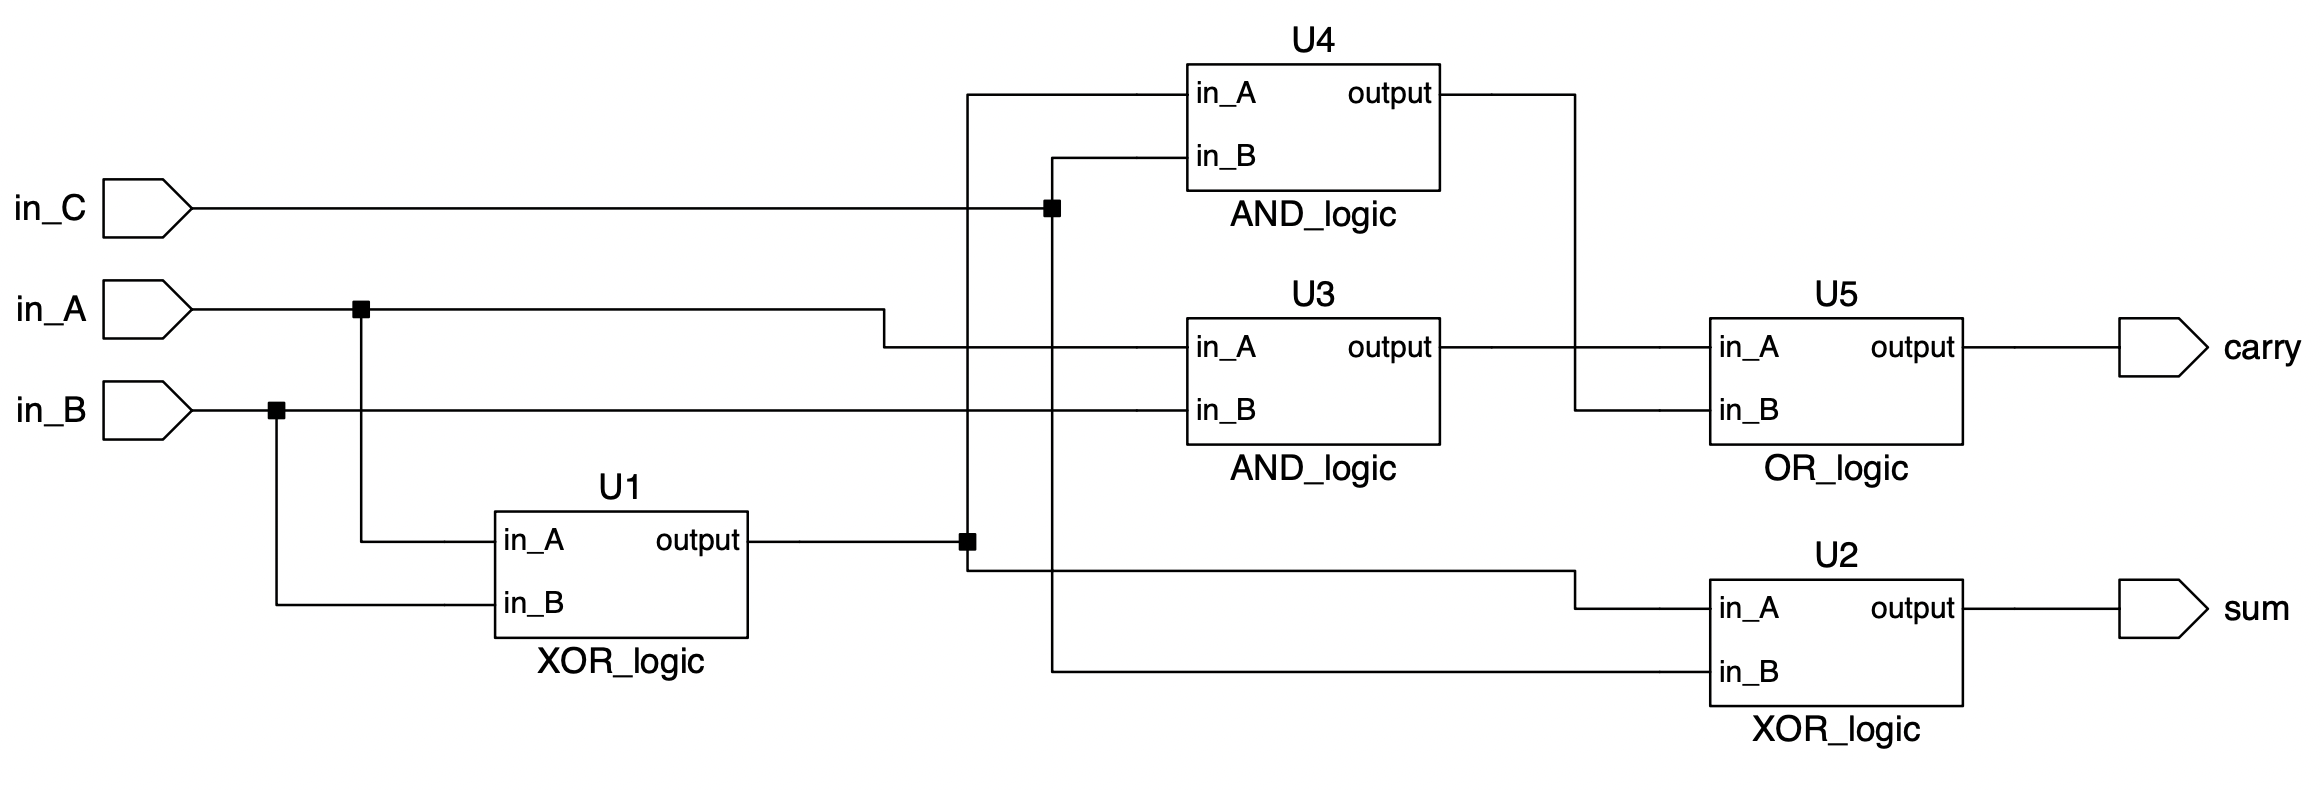
\includegraphics[width=0.9\textwidth]{../img/fa_rtl.png}
	\label{fig:fa_rtl}
\end{figure}

\noindent The simulation results for the full adder are shown in \figref{fig:fa_sim}.

\begin{figure}[!ht]
	\centering
	\caption{Simulation Wave Diagram of Full Adder Block}
	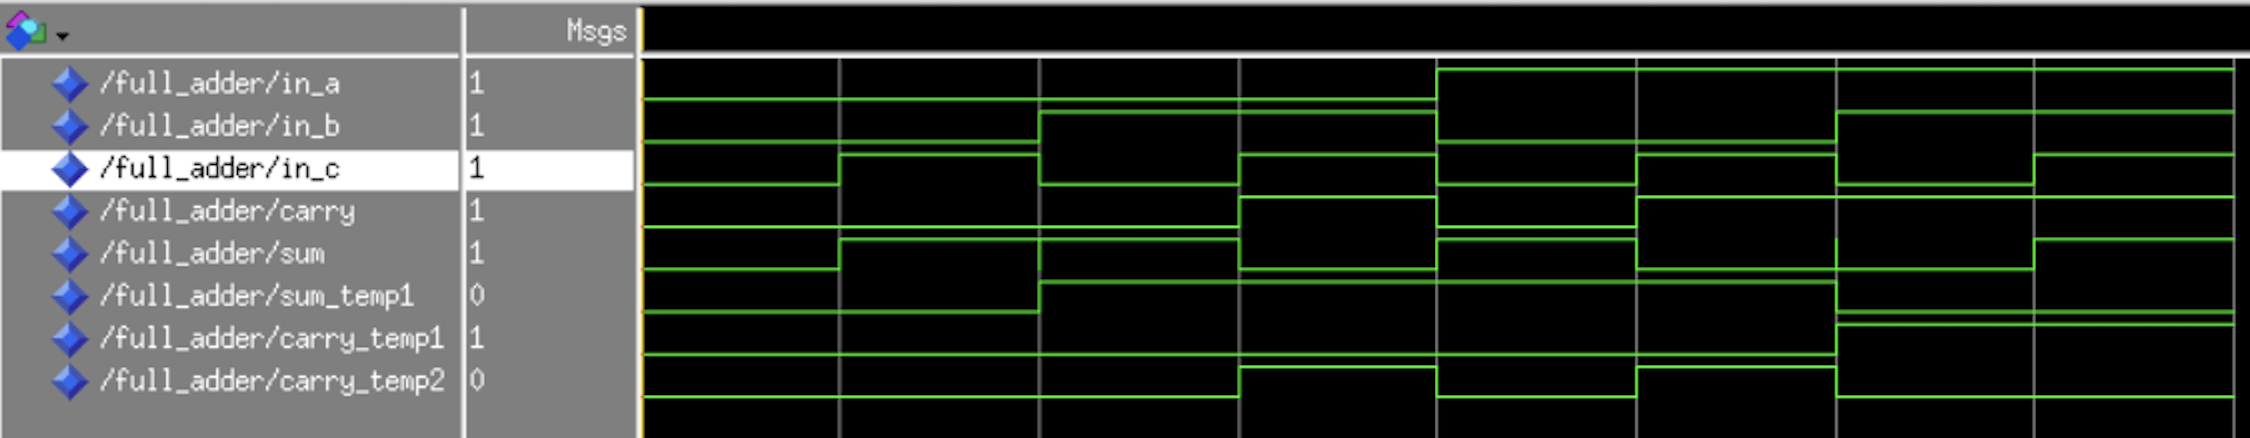
\includegraphics[width=0.9\textwidth]{../img/fa_sim.png}
	\label{fig:fa_sim}
\end{figure}

\subsection{Two to one multiplexer}

The 2-to-1 multiplexer is a selector that has a switch to control the input, the circuit which consists of \textbf{AND} gate, \textbf{OR} gate and \textbf{NOT} gate.
For a 2-to-1 multiplexer, the inputs are \(A\) and \(B\), \(Sel\) is the select signal and \(Z\) is the output.
Depending on the select signal, the output is connected to either of the inputs.
If \(Sel = 0\), then the output will be switched to input a, whereas if \(Sel = 1\), then the output will be switched to input b.
The truth table is shown in \tbref{tb:mx_boo}.

\begin{table}[!ht]
	\renewcommand{\arraystretch}{0.7}
	\caption{2-to-1 Multiplexer Truth Table}
	\centering
	\begin{tabular}{ >{\centering\arraybackslash}p{2cm} >{\centering\arraybackslash}p{2cm} >{\centering\arraybackslash}p{2cm} | >{\centering\arraybackslash}p{2cm} }
		\hline
		\bfseries A & \bfseries B & \bfseries Select & \bfseries Output \\
		\hline
		0           & -           & 0                & 0                \\
		1           & -           & 0                & 1                \\
		-           & 0           & 1                & 0                \\
		-           & 1           & 1                & 1                \\
		\hline
	\end{tabular}
	\label{tb:mx_boo}
\end{table}

\noindent The equation for the multiplexer is defined at \expref{exp:mx_exp}

\begin{equation}
	\begin{array}{c}
		Y=(\overline{Sel} \bullet  A )+( Sel\bullet B )
	\end{array}
	\label{exp:mx_exp}
\end{equation}

\noindent The circuit for the multiplexer is shown in \figref{fig:mx_rtl}.

\noindent The simulation results for the multiplexer are shown in \figref{fig:mx_sim}.

\begin{figure}[!htp]
	\centering
	\caption{Synthesized RTL Diagram of 2-to-1 Multiplexer Block}
	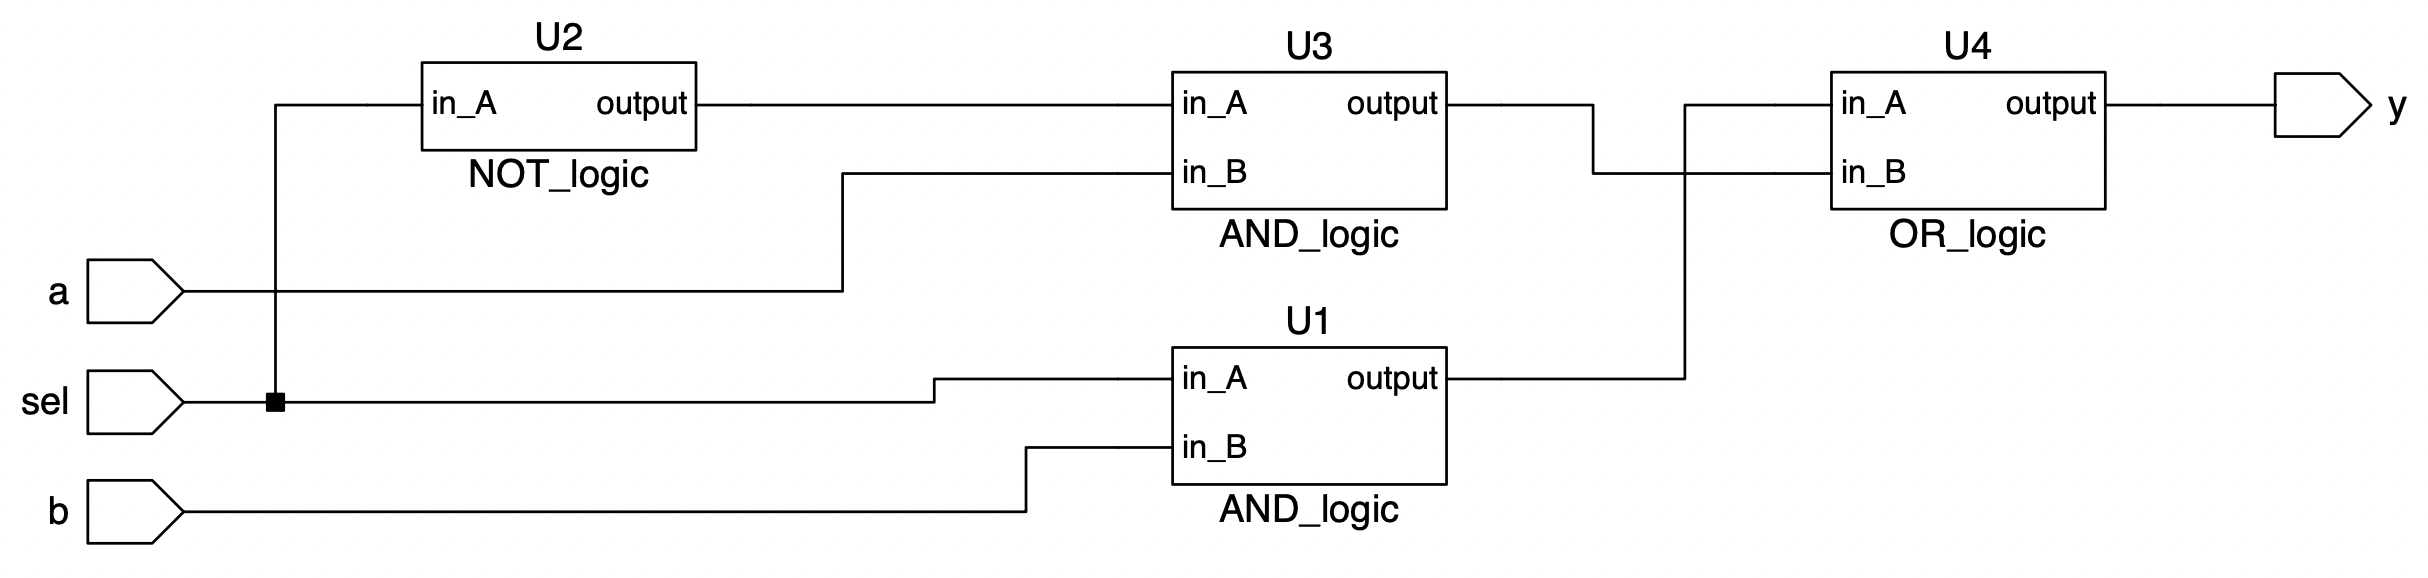
\includegraphics[width=0.9\textwidth]{../img/mx_rtl.png}
	\label{fig:mx_rtl}
\end{figure}


\begin{figure}[!htp]
	\centering
	\caption{Simulation Wave Diagram of 2-to-1 Multiplexer Block}
	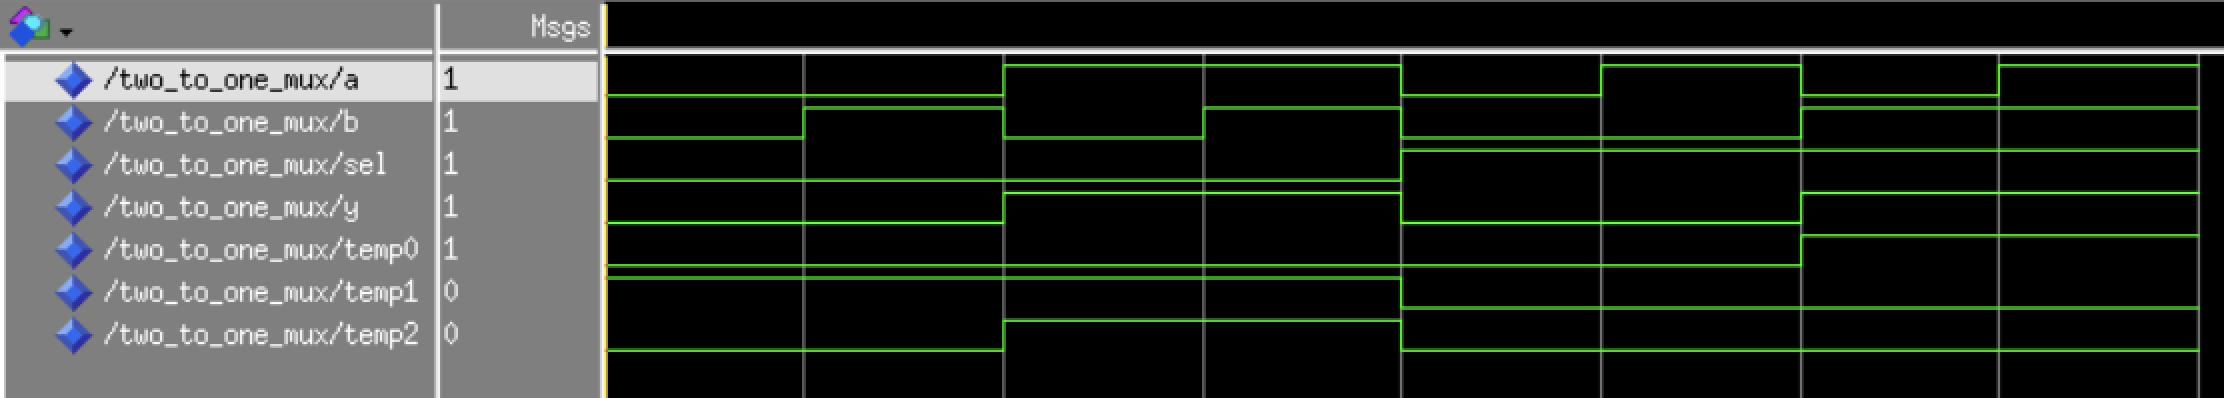
\includegraphics[width=0.9\textwidth]{../img/mx_sim.png}
	\label{fig:mx_sim}
\end{figure}

\subsection{4-bit Ripple Carry Adder}

In order to build n-bit carry select adders which are suitable for this project,
a 4-bit ripple carry adder block is the basic component.
A ripple carry adder is cascaded in parallel by multiple full adder circuits,
in which the carry out of each full adder is the carry in of the succeeding next most significant full adder.
Four full adders are tied together to build the 4-bit ripple carry adder block for this project.
Where \(A\) and \(B\) are 4-bit inputs, sum is the addition output of \(A\) and \(B\), \(Carry_{out}\) is the output carry which depends on \(C_{in}\), \(C_1\), \(C_2\), \(C_3\).
The circuit for the 4-bit ripple carry adder block is shown in \figref{fig:rca_rtl}.

\begin{figure}[!htp]
	\centering
	\caption{Synthesized RTL Diagram of 4-bit Ripple Carry Adder Block}
	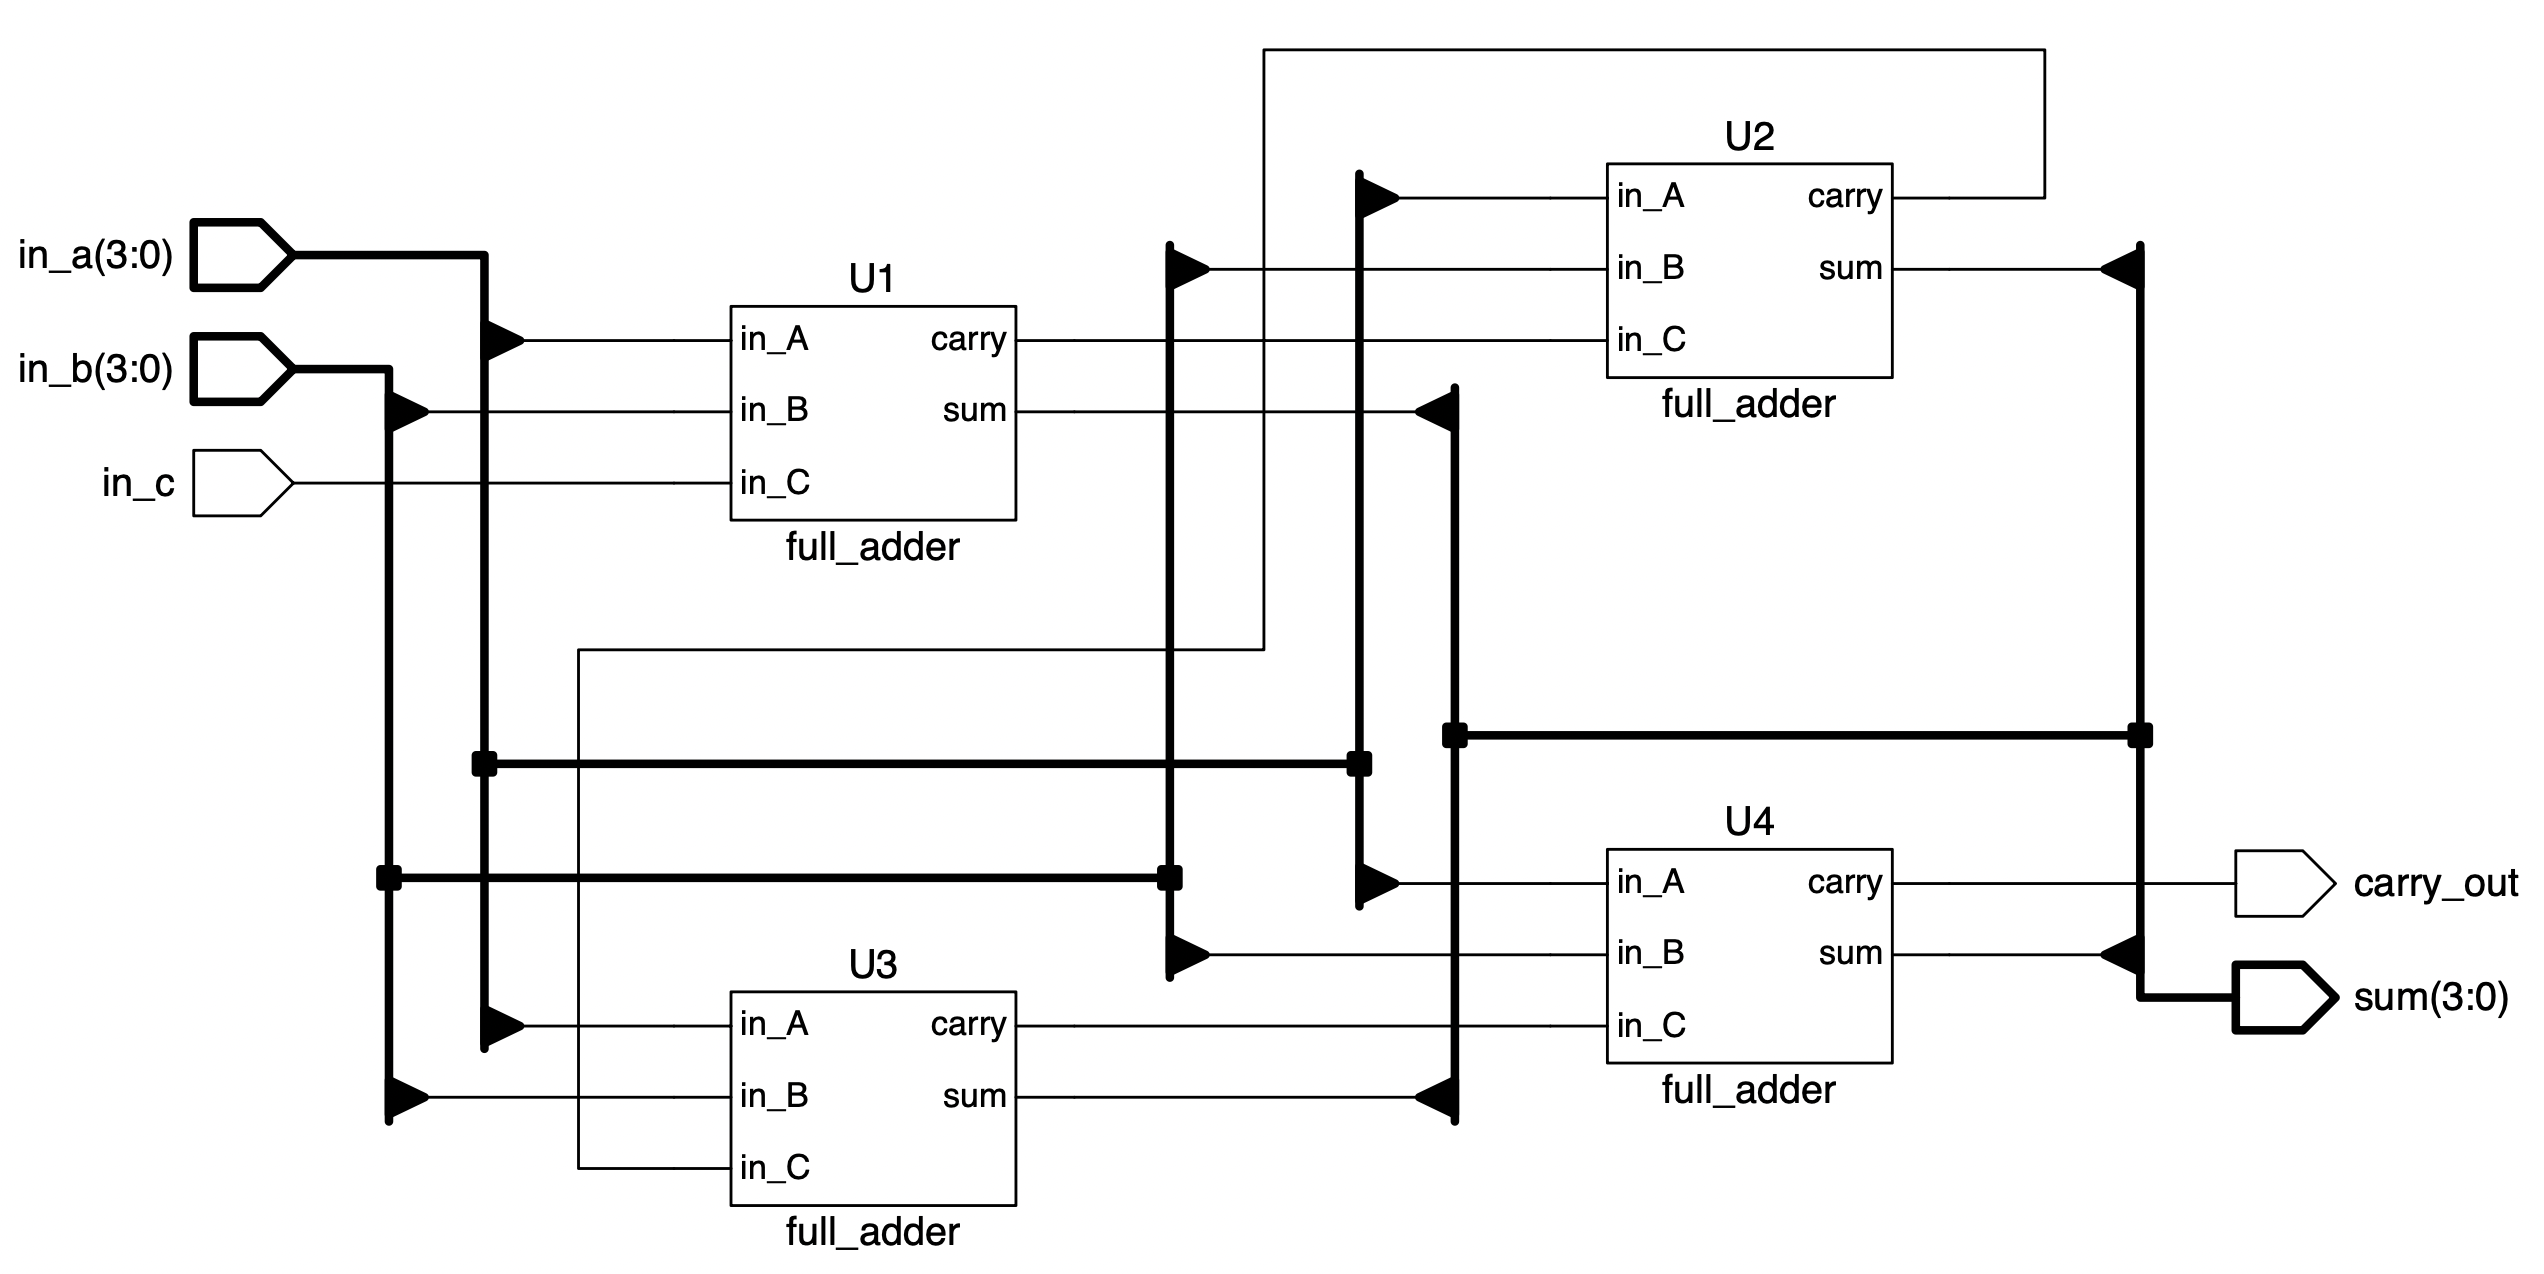
\includegraphics[width=0.9\textwidth]{../img/rca_rtl.png}
	\label{fig:rca_rtl}
\end{figure}

\noindent The selected simulation cases are shown below and the simulation results for the 4-bit ripple carry adder are shown in \figref{fig:rca_sim}.
\begin{itemize}
	\item A general purpose test addition
	\item Overflow test
	\item Zeros test
\end{itemize}

\begin{figure}[!htp]
	\centering
	\caption{Simulation Wave Diagram of 4-bit Ripple Carry Adder Block}
	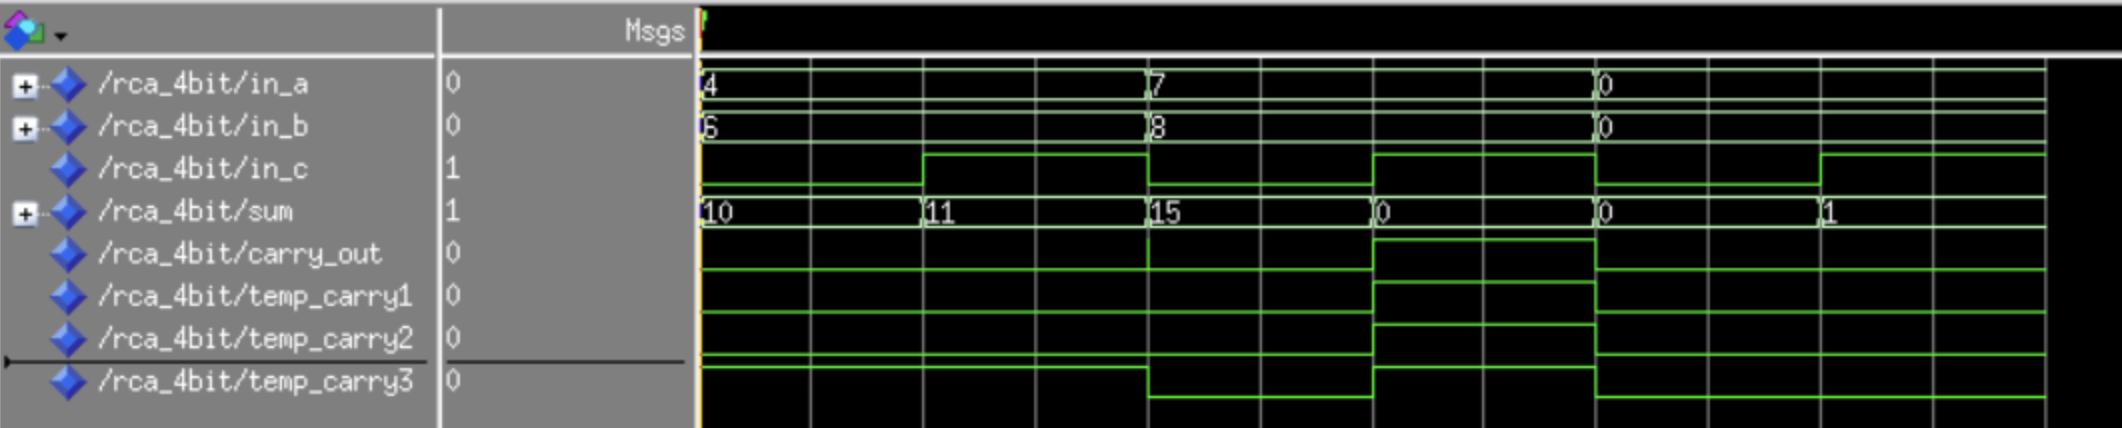
\includegraphics[width=0.9\textwidth]{../img/rca_sim.png}
	\label{fig:rca_sim}
\end{figure}

\subsection{4-bit Carry Select Adder}

A basic building block size of carry select adder is four.
A 4-bit carry select adder consists of two parallel 4-bit ripple carry adders and 2-to-1 multiplexers to perform the calculation twice.
One of the 4-bit RCA block assumes that the input carry is 0 (RCA\_0), the other assumes that the input carry is 1 (RCA\_1).
After the two results are calculated, the correct sum, as well as the correct carry out, is then selected with the multiplexer once the correct carry in is known.
The delay equation for the 4-bit carry select adder is defined below:

\begin{equation}
	\begin{array}{c}
		T_{CSA} = T_{mux} + 4 \times T_{full\_adder}
	\end{array}
	\label{exp:csa_delay_exp}
\end{equation}

\noindent The circuit for the 4-bit carry select adder is shown in \figref{fig:csa_4_rtl}.

\begin{figure}[!htp]
	\centering
	\caption{Synthesized RTL Diagram of 4-bit Carry Select Adder Block}
	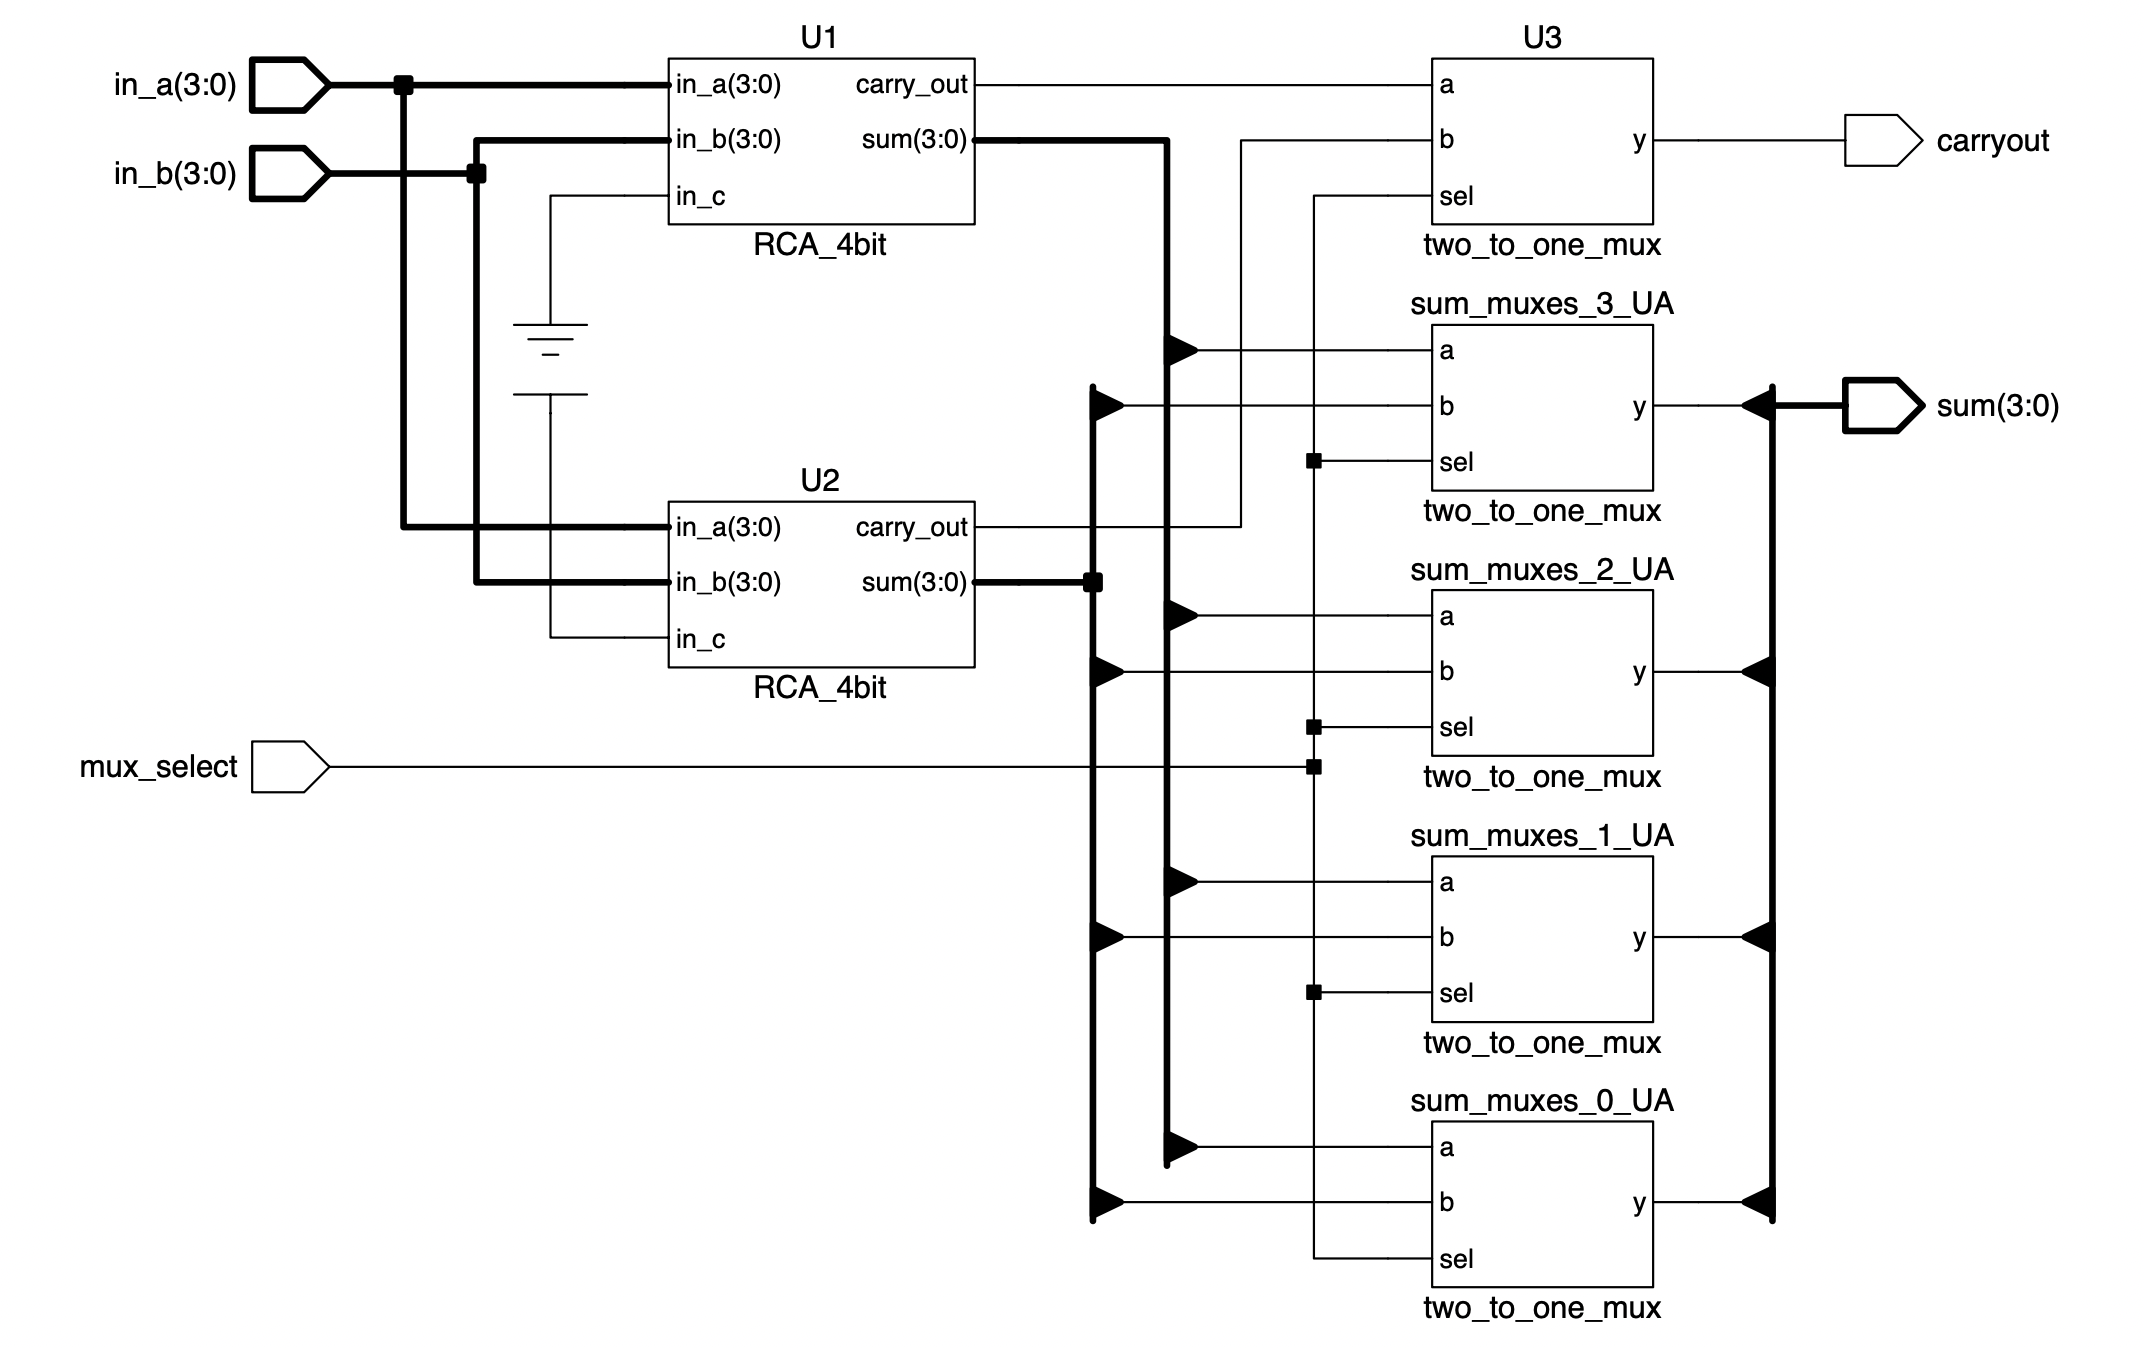
\includegraphics[width=0.9\textwidth]{../img/csa_4_rtl.png}
	\label{fig:csa_4_rtl}
\end{figure}
If the input carry \(C_{in}\) from the lower level is 0, the output carry of the RCA\_0 is selected as the output carry of this 4-bit CSA block.
If the input carry \(C_{in}\) from the lower level is 1, the output carry of the RCA\_1 is selected as the output carry.
At the same time \(C_{in}\) is used as the selection signal of 2-to-1 multiplexer to control whether the output of S3 to S0 comes from the RCA\_0 or the RCA\_1.

\noindent The simulation results for the 4-bit carry select adder are shown in \figref{fig:csa_4_sim}.

\begin{figure}[!htp]
	\centering
	\caption{Simulation Wave Diagram of 4-bit Carry Select Adder Block}
	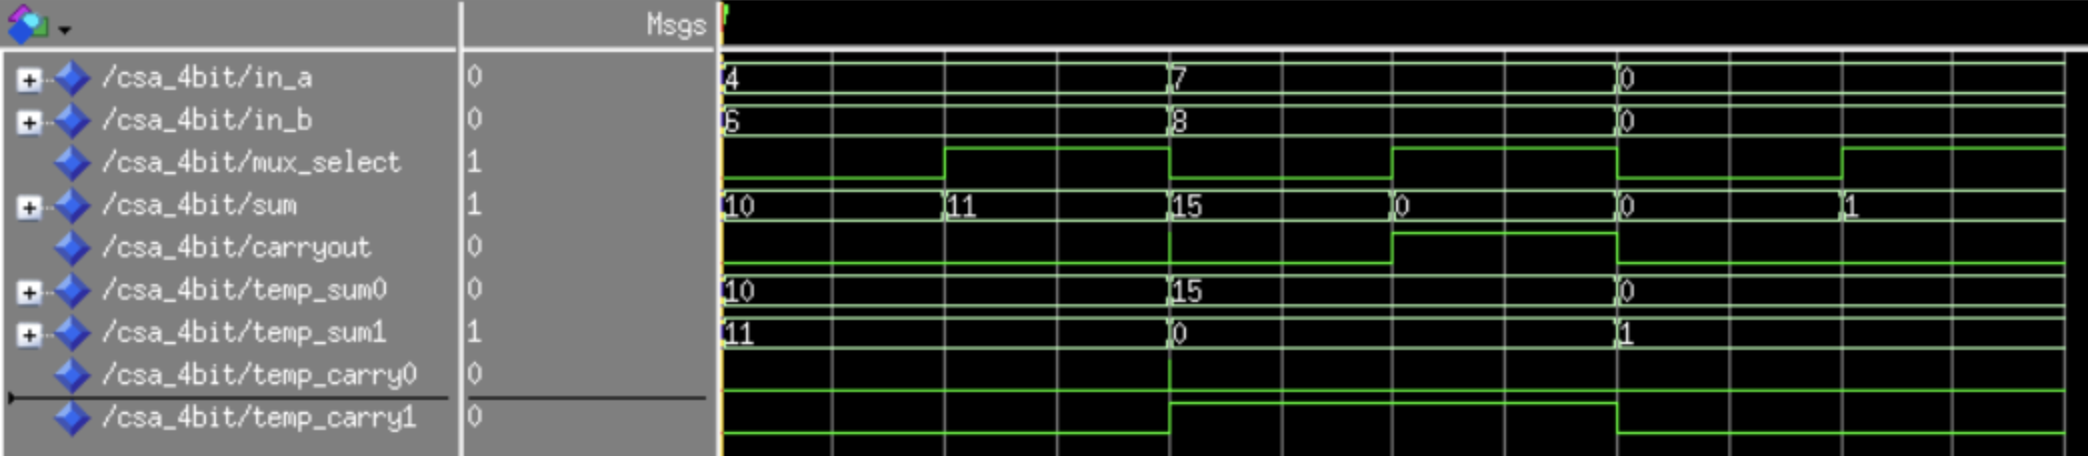
\includegraphics[width=0.9\textwidth]{../img/csa_4_sim.png}
	\label{fig:csa_4_sim}
\end{figure}

\newpage

\subsection{16-bit Carry Select Adder}

In this project, 16-bit carry select adder is used.
A 16-bit carry select adder can be created using three 4-bit CSA blocks and one 4-bit RCA blocks.
The first block is a 4-bit RCA, the inputs are two binary numbers from multiplier, so that there is no input carry and the \(C_{in}\) can be set to 0.
Then the delay of this adder will be the delay of the four full adders, plus the delay of the three MUXs.
The delay equation for the 16-bit carry select adder is defined below:

\begin{equation}
	\begin{array}{c}
		T_{CSA} = 3 \times T_{mux} + 4 \times T_{full\_adder}
	\end{array}
	\label{exp:csa_16b_delay_exp}
\end{equation}

\noindent The circuit for the 16-bit carry select adder is shown in \figref{fig:csa_16_rtl}.

\begin{figure}[!htp]
	\centering
	\caption{Synthesized RTL Diagram of 16-bit Carry Select Adder Block}
	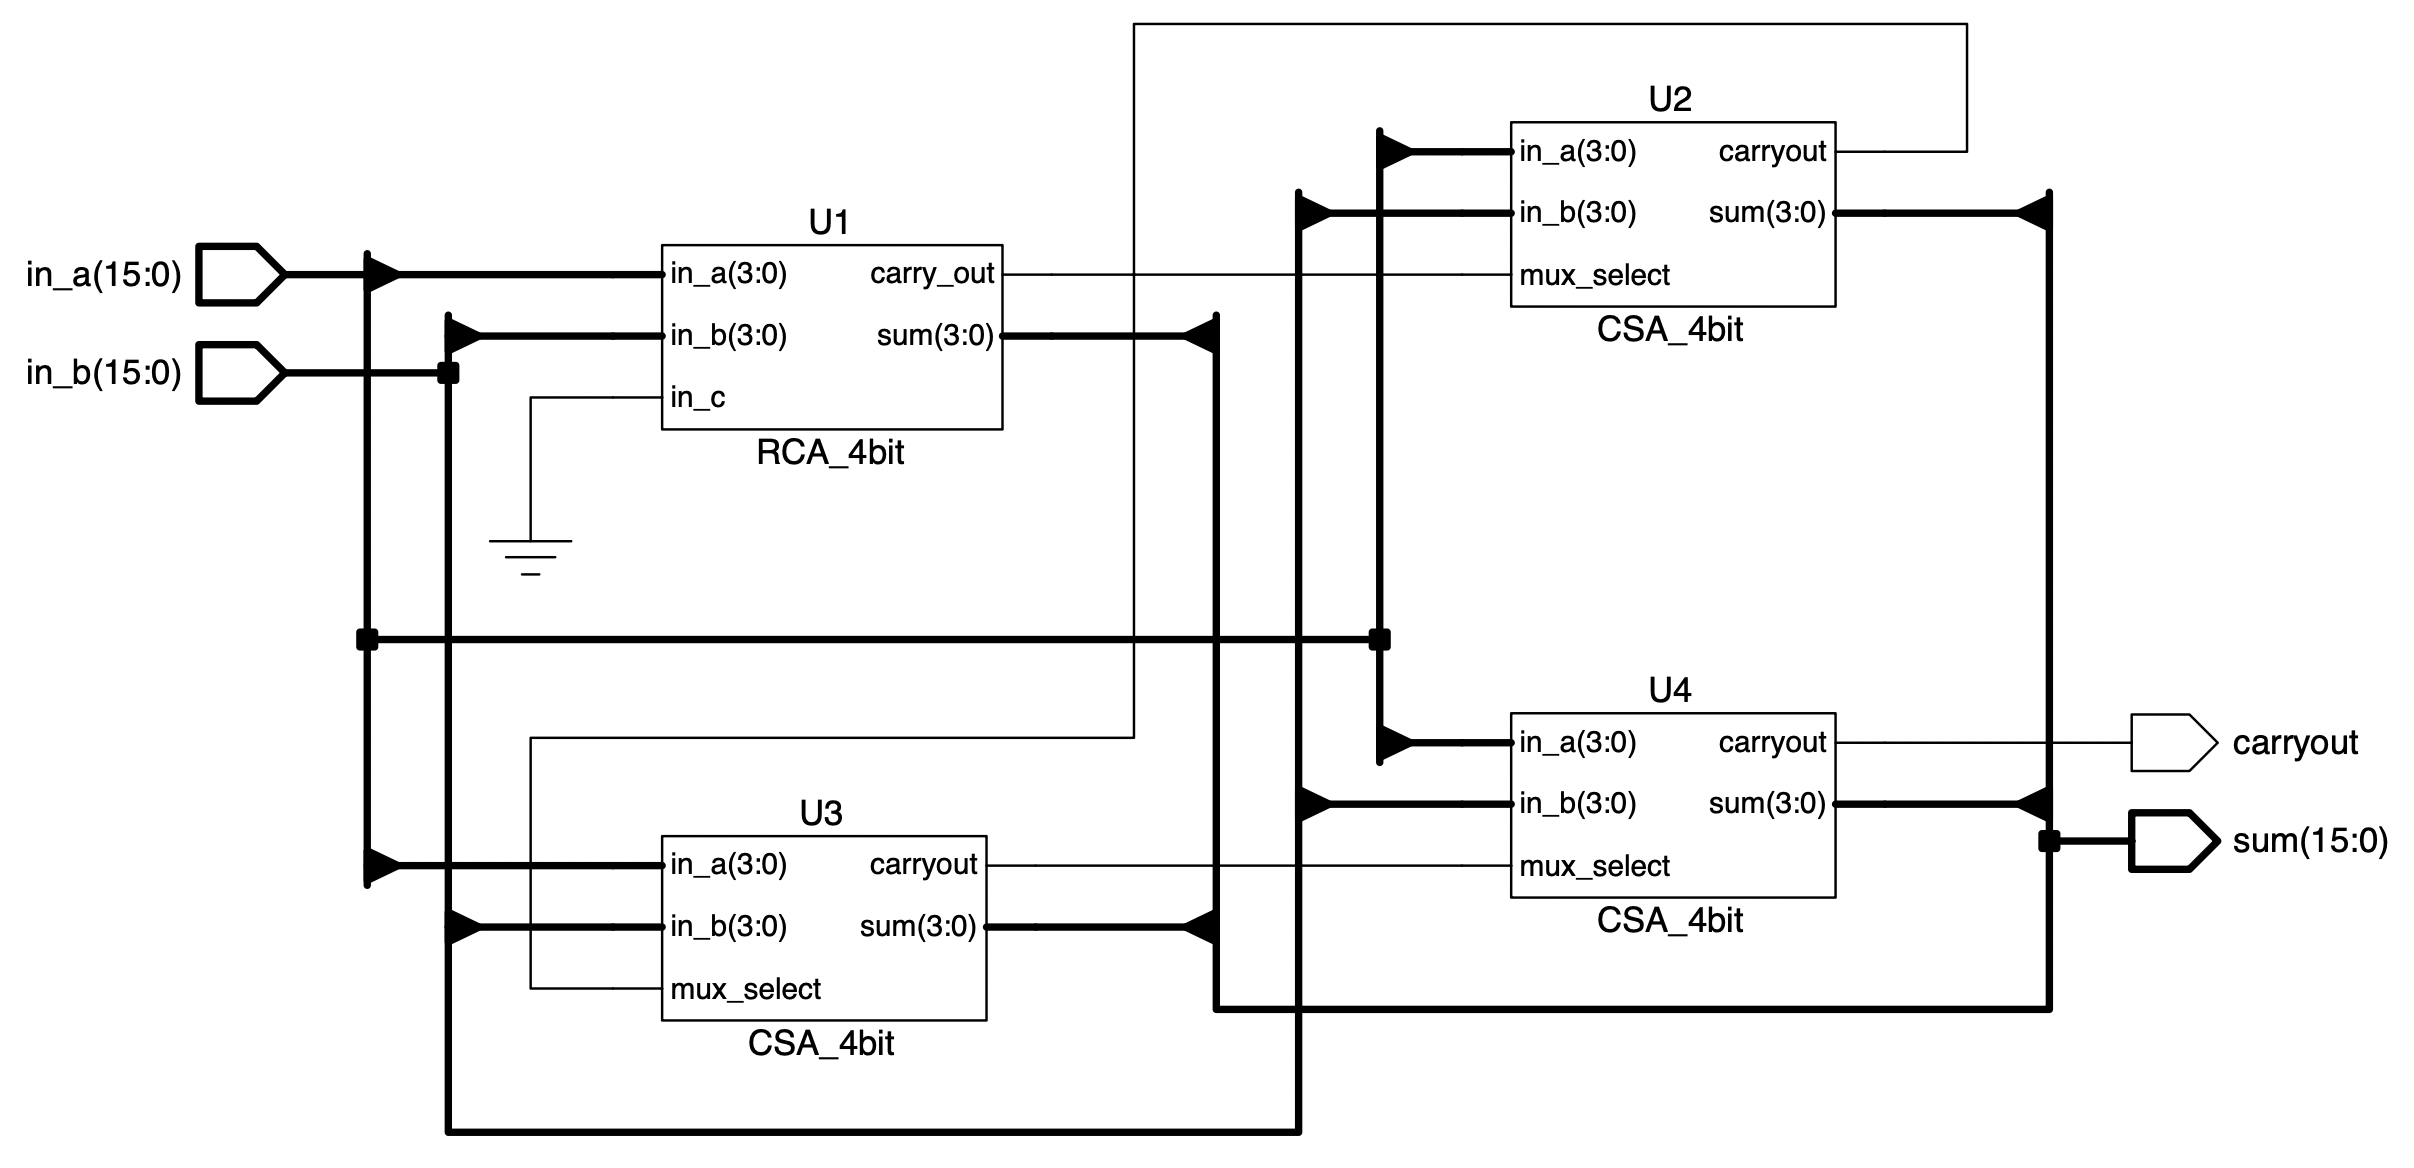
\includegraphics[width=\textwidth]{../img/csa_16_rtl.png}
	\label{fig:csa_16_rtl}
\end{figure}

\noindent The simulation results for the 16-bit carry select adder are shown in \figref{fig:csa_16_sim}.

\begin{figure}[!htp]
	\centering
	\caption{Simulation Wave Diagram of 16-bit Carry Select Adder Block}
	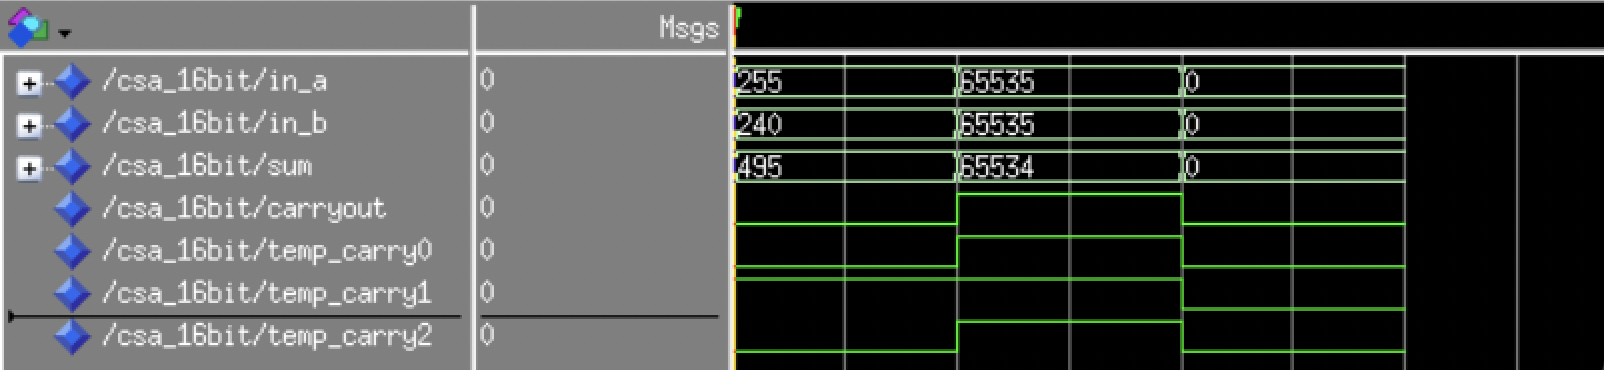
\includegraphics[width=0.8\textwidth]{../img/csa_16_sim.png}
	\label{fig:csa_16_sim}
\end{figure}

\subsection{24-bit Carry Select Adder}


Same principle as a 16-bit CSA, a 24-bit CSA is built up with five 4-bit CSA blocks and one 4-bit RCA block.
Also, the first block is 4-bit RCA, the inputs are two binary numbers from multiplier,
so that there is no input carry and the \(C_[in]\) can be set to 0.
The delay equation for the 16-bit carry select adder is defined below:

\begin{equation}
	\begin{array}{c}
		T_{CSA} = 5 \times T_{mux} + 4 \times T_{full\_adder}
	\end{array}
	\label{exp:csa_24b_delay_exp}
\end{equation}

\noindent The circuit for the 24-bit carry select adder is shown in \figref{fig:csa_16_rtl}.

\begin{figure}[!htp]
	\centering
	\caption{Synthesized RTL Diagram of 24-bit Carry Select Adder Block}
	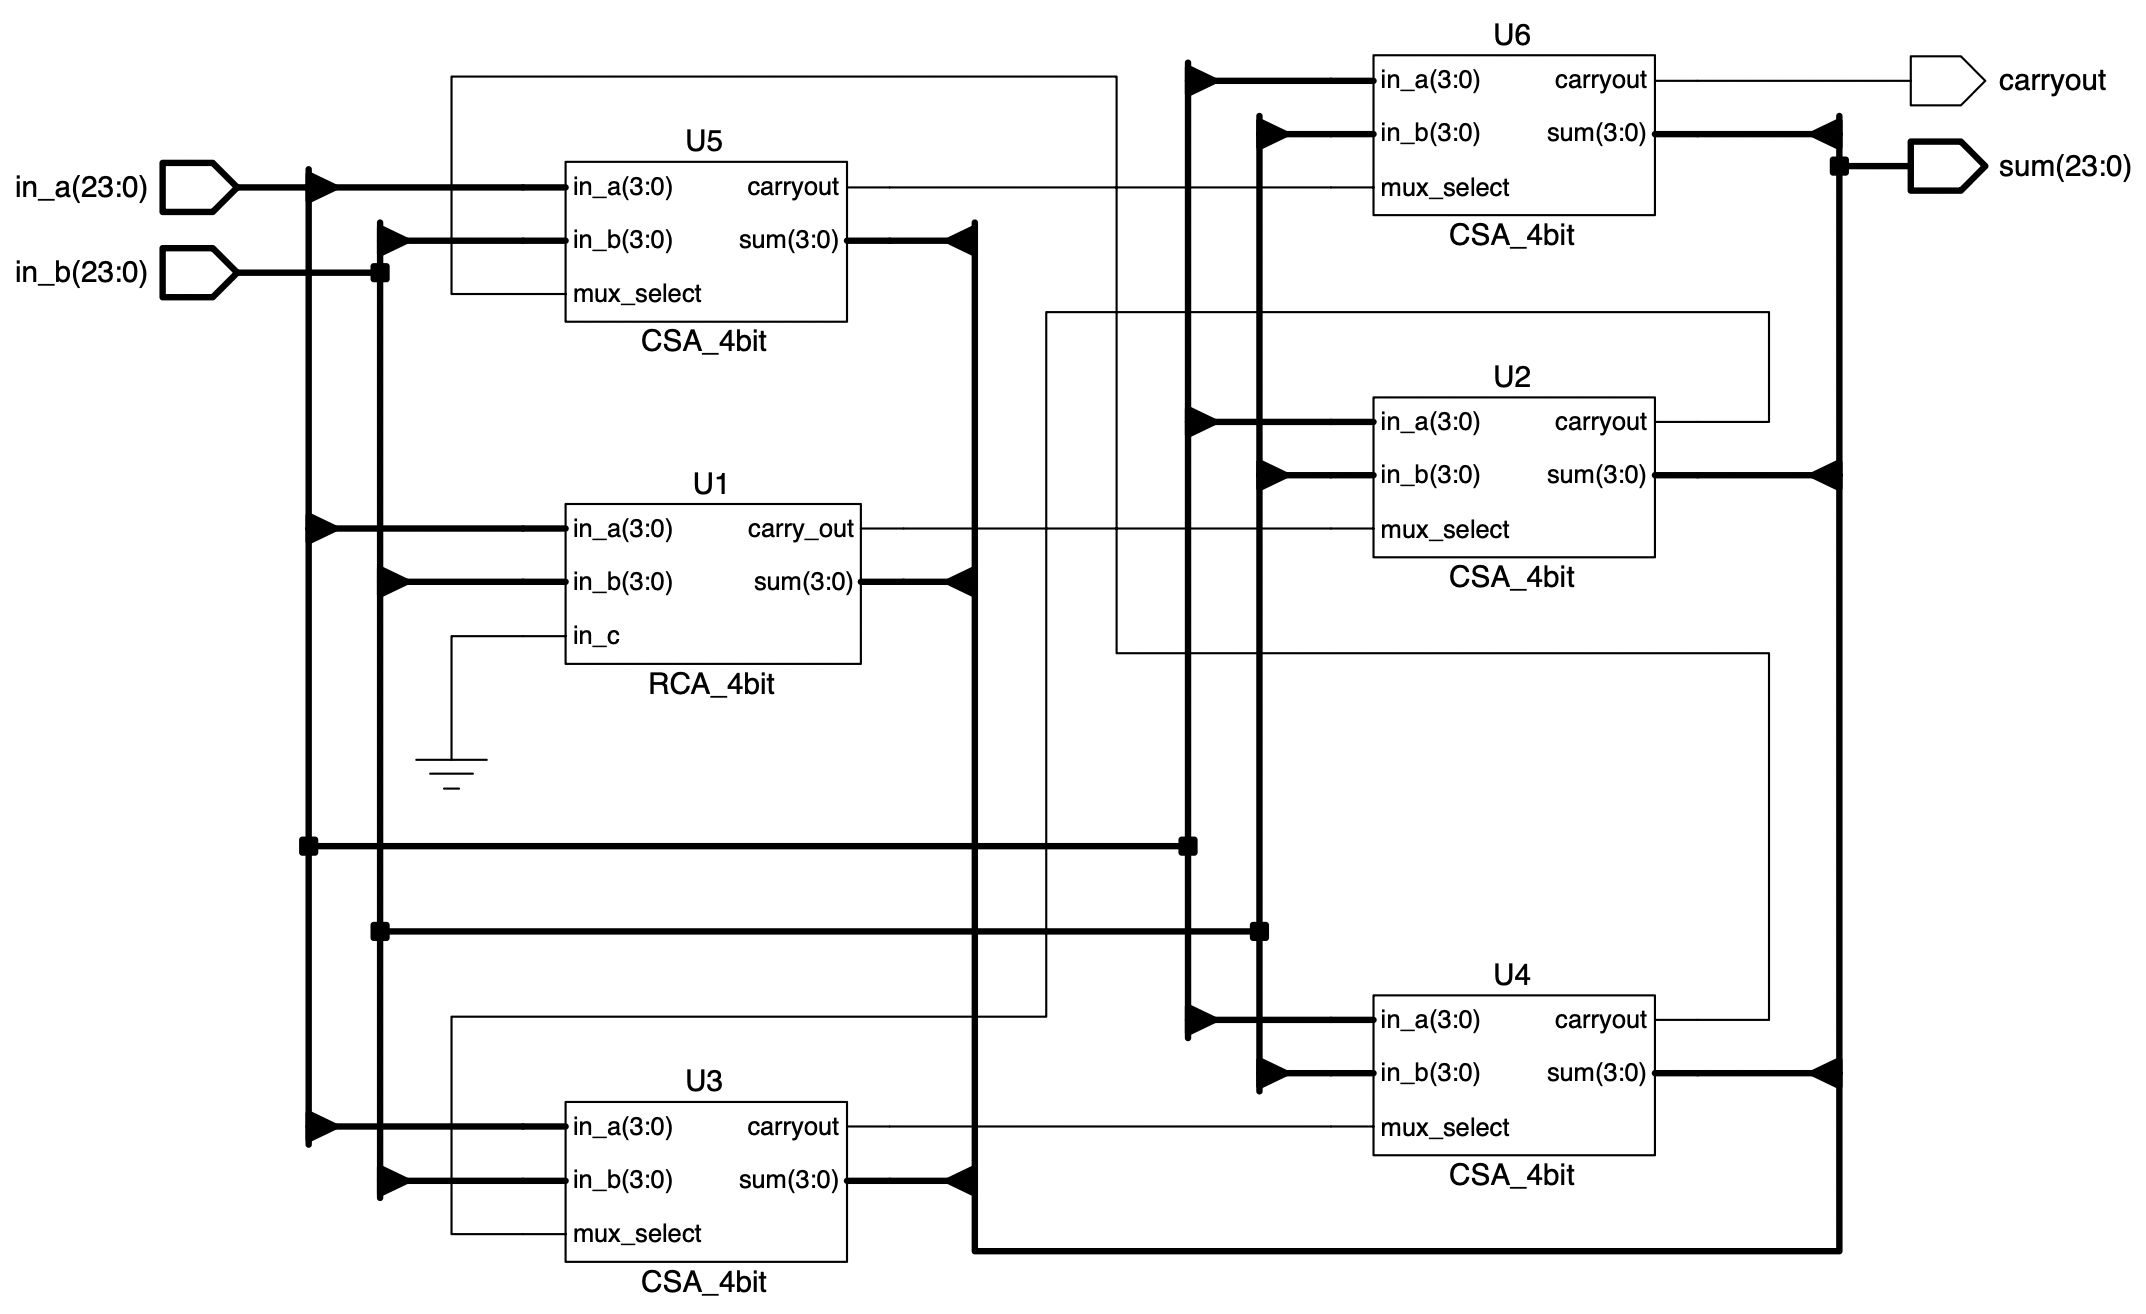
\includegraphics[width=0.9\textwidth]{../img/csa_24_rtl.png}
	\label{fig:csa_24_rtl}
\end{figure}

\noindent The simulation results for the 24-bit carry select adder are shown in \figref{fig:csa_24_sim}.

\begin{figure}[!htp]
	\centering
	\caption{Simulation Wave Diagram of 24-bit Carry Select Adder Block}
	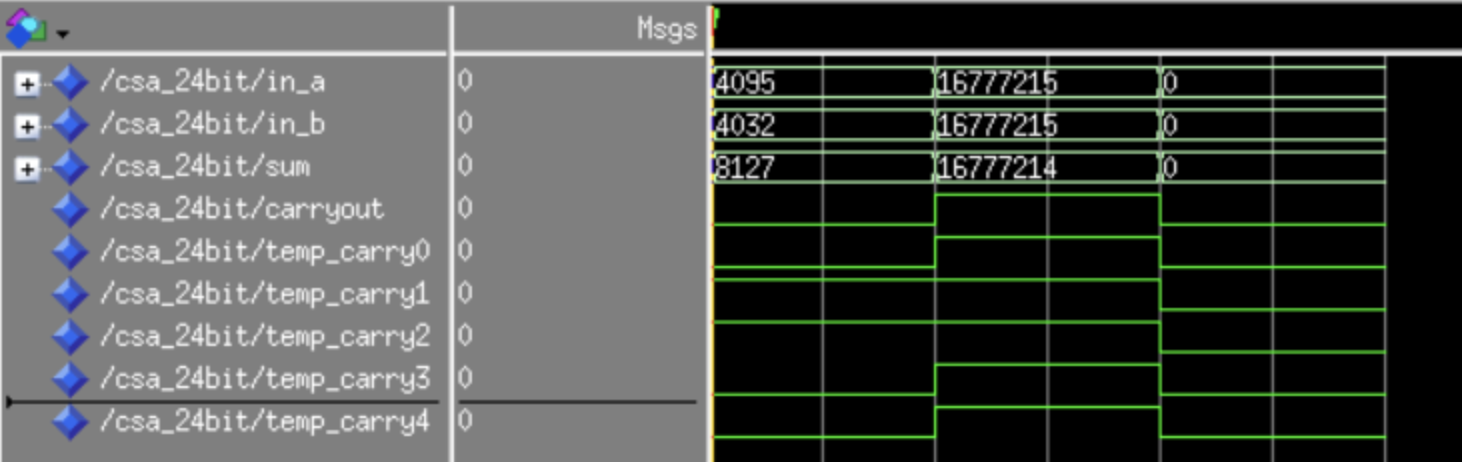
\includegraphics[width=0.8\textwidth]{../img/csa_24_sim.png}
	\label{fig:csa_24_sim}
\end{figure}

\subsection{24-bit CSA Incrementor}

The incrementor used in this project were designed on the basis of the CSA.
The principle is to define the input B of the CSA as a constant with the lowest bit of 1 and the rest of 0.
Due to different bit requirements, a N-bit incrementor can be implemented by N-bit CSA.
A 24-bit incrementor is used in this project.
The circuit for the 24-bit incrementor is shown in \figref{fig:24_incre_rtl}.

\begin{figure}[!htp]
	\centering
	\caption{Synthesized RTL Diagram of 24-bit Incrementor Block}
	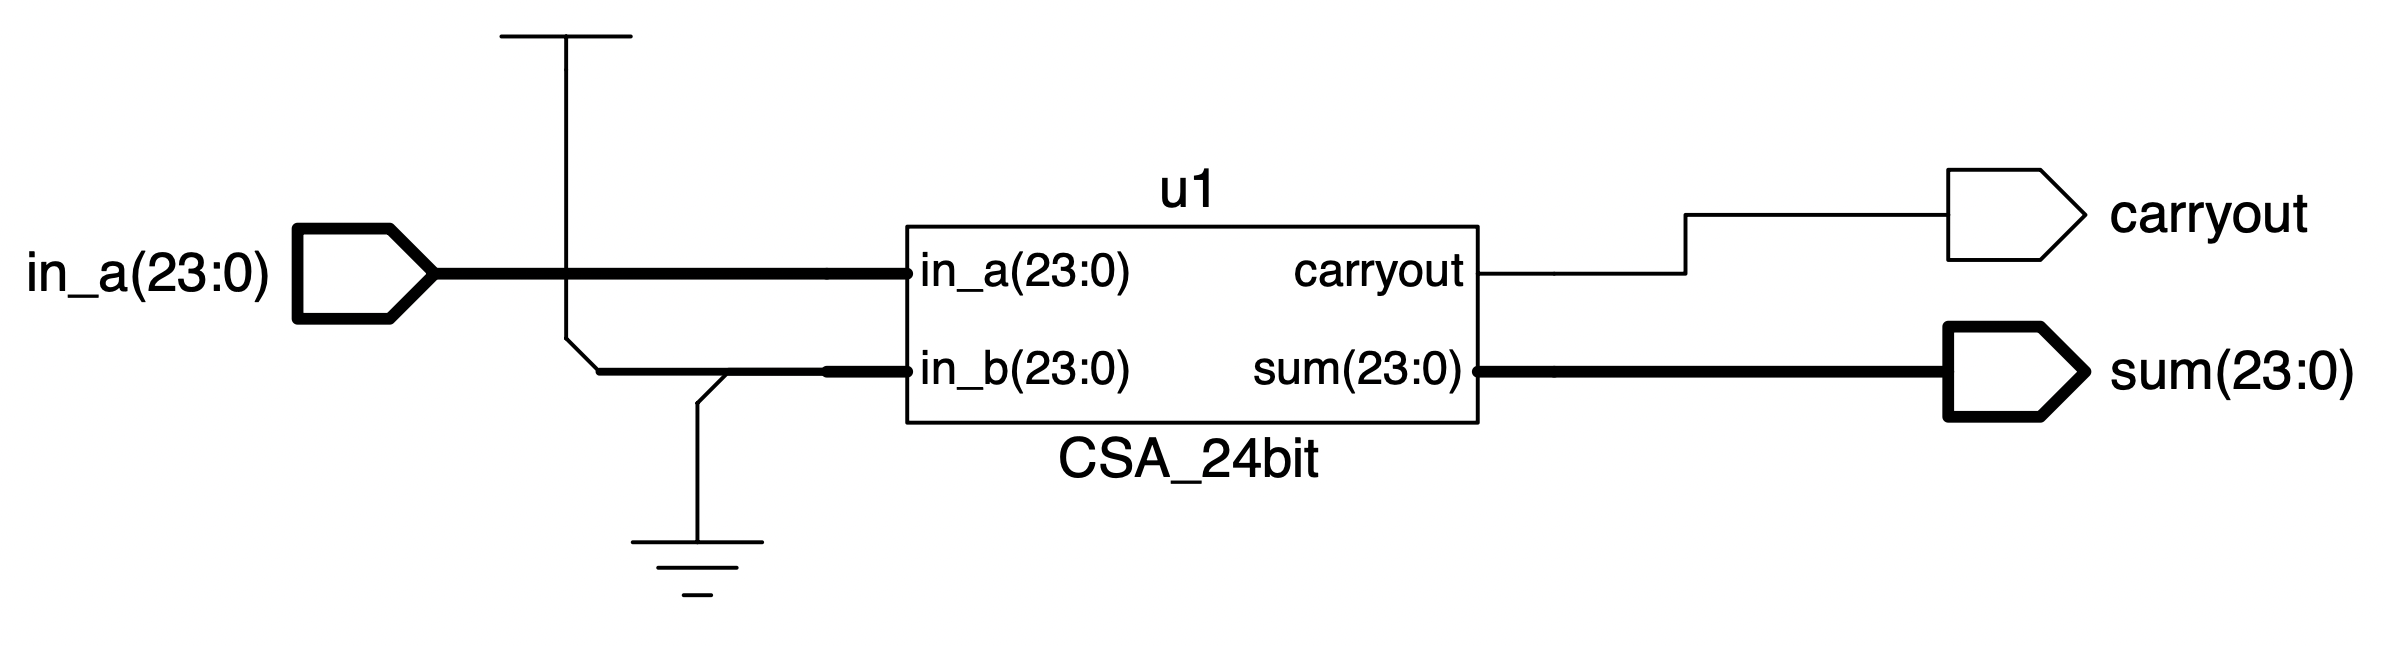
\includegraphics[width=0.9\textwidth]{../img/24_incre_rtl.png}
	\label{fig:24_incre_rtl}
\end{figure}

The simulation results for the 24-bit incrementor are shown in \figref{fig:24_incre_sim}.

\begin{figure}[!htp]
	\centering
	\caption{Simulation Wave Diagram of 24-bit Incrementor Block}
	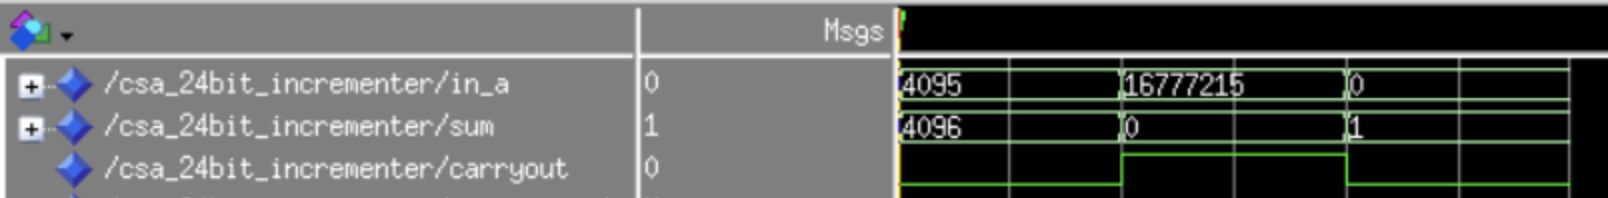
\includegraphics[width=0.9\textwidth]{../img/24_incre_sim.png}
	\label{fig:24_incre_sim}
\end{figure}